\section{Evaluation}\label{sec:eval}
In this chapter we will evaluate the presented approaches by using the trained models from Chapter~\ref{sec:multi-task-ft} and \ref{sec:single-task-ft} to extract event logs from patient journeys. In order to properly compare the fine-tuned models and the base model, we will first introduce the metrics we use. Second, we will describe the evaluation process. Third, we will present our results for each model, each task and each of the task's metrics individually.\\
The evaluation is based on comparing the extracted event logs to a ground truth and determining the differences between them. This is one out of a few options already established in the academic context~\cite{latif_fine-tuning_2024}.

\subsection{Metrics}\label{sec:metrics}
In \ref{sec:multi-task-ft} we describe the process of fine-tuning a model to perform multiple related tasks. We evaluate each of these tasks individually. The model trained in \ref{sec:single-task-ft} performs only the task \quotes{Activity Labeling}, so we use the metric described in \ref{sec:activity_metrics} as well.

\subsubsection{Activity Labelling Metrics}\label{sec:activity_metrics}
There already are established metrics in the process mining sector we can use to determine if an event log is of good quality in terms of activities.~\cite{van_der_aalst_process_2016, carmona_conformance_2018} They propose three categories an activity can have. We use similar categories for the activity labels.\\
It is worth noting, that determining if one activity label from the evaluated event log and one from the ground truth are indeed the same activity label is not as straight forward as one might think. As discussed in \ref{sec:tracex}, the activity labels are not predetermined, instead they are chosen by the model that extracts them. This means two activity labels can be syntactically different but still describe the same activity. For the purpose of this evaluation, we define two activity labels as identical, if they are semantically very similar.
\paragraph{Missing Activity} An activity is missing, if it is featured in the ground truth, but not in the evaluated event log. 
\paragraph{Unexpected Activity} An activity is unexpected, if it is featured in the evaluated event log, but not in the ground truth.
\paragraph{Wrong Order} Two activities are in wrong order, if both of them are featured in the ground truth as well as the evaluated event log, but their order of appearance is interchanged. In our case, the order of activities is defined by their start timestamp. This means two activities $A_1 \text{ and } A_2$ are in wrong order, if they appear in the order $A_1,A_2$ in the ground truth and in order $A_2, A_1$ in the evaluated event log.\\\\
As this is a comparative analysis, the value we use from this metric is the percentage of errors in each of the mentioned categories – Missing Activity, Unexpected Activity and Wrong order. This way, the number of errors is relative to the number of activities in the respective patient journey.

\subsubsection{Event Type Classification Metric}\label{sec:eventtype_metric}
We use a set of event types so each pair of them is mutually exclusive. This means for every activity in the ground truth there is exactly one correct event type. This fact reduces this metric to two possible results per event type: \emph{True} and \emph{False.}\\
The value we use from this metric is the percentage of \verb|True| and \verb|False| values respectively. This way, the number of errors is relative to the number of activities in the respective patient journey.\\
Possible event types are: Symptom Onset, Symptom Offset, Doctor Visit. Hospital Admission, Hospital Discharge, Treatment, Medication, Lifestyle Change, Feelings.

\subsubsection{Timestamp Extraction Metrics}\label{sec:time_metrics}
Similar to the event type metric, a timestamp can be either extracted correctly or incorrectly, resulting in \verb|True| or \verb|False| when evaluated. In order to adhere to the commonly used standard in event logs, that is also required to produce valid XES files, the timestamps are in the format \verb|YYYY-MM-DD|. In many cases, including the sample patient journeys we use in the evaluation, patient journeys do not contain time information this precise. Most time specifications are relative and vague. For the purpose of this evaluation, we define a timestamp to extracted correctly, if the date is plausible in the context of the patient journey. For an activity, that is described to have happened on \quotes{some day in April…}, any timestamp between 01.~April and 30.~April would be correct. This is, unless there is other time related information that further specifies the timeframe in which an activity must have happened. Let $A_1$ be an activity that happens before activity $A_2$ and $t_2=$ \verb|2024-04-15q| be the timestamp for $A_2$. If $A_1$ is specified as \quotes{some day in April…}, only timestamps between 01.~April and 14.~April would be correct. The same goes for \quotes{as the weeks progressed}, \quotes{later that year} and similar phrases. As long as an extracted timestamp is correct relatively to all other information given in the patient journey and is as precise as the text provides, it is deemed correct.\\
Start and end timestamps can be correct or incorrect independent of each other. The value we use from this metric is the percentage of \verb|True| and \verb|False| values respectively. This way, the number of errors is relative to the number of activities in the respective patient journey.

\subsection{Evaluation Process}\label{sec:eval_process}
In this chapter we will describe the process of evaluating the models trained in Chapter~\ref{sec:multi-task-ft} and \ref{sec:single-task-ft} using the metrics proposed in chapter \ref{sec:metrics}.\\
In order to evaluate the quality of the extraction performed by the various models, we need Patient Journeys to extract event logs from. First, we assemble a collection of Patient Journeys that pose different challenges. They are listed in full length in the appendix at \ref{apx:pjs}. They include well-structured descriptions of consecutive events and explicitly stated time stamps, but also implied activities and events with strong temporal relations that are not easily understood without taking a big context window into account. In short – the sample patient journeys provide a diverse mix of challenges, featuring both easy and hard to extract information.\\
We want to conduct comparative analyses between LLM models. To make these as fair and deterministic as possible, the next step is to create ground truths for every patient journey and every task that is performed on them. They can be found in the appendix at \ref{apx:ground_truths}. We later on use the same Patient Journeys and respective ground truths for all models.\\
The extraction itself is done using the TracEX pipeline. To address the dependency of the Event Type Classification step detailed in \ref{sec:back} we inject the activities from the ground truth into the pipeline before executing that step. This ensures that no previous step affects the results of the extraction in an uncontrolled way.\\\\
The extraction uses LLMs, which are non-deterministic by design. Due to that fact, the results vary between executions, even with the same input. To solve this issue, we perform each execution multiple times and use the mean of all values between the executions for the evaluation. All datasets without the mean calculation can be found in the appendix at \autoref{apx:pipeline}.\\\\
As mentioned in \autoref{sec:tracex} TracEX uses Few-Shot prompts for every task we examine in this thesis. The fine-tuned model will perform all tasks without the additional examples in the few-shot prompts, since the training data should suffice to convey what is demanded from the model.

\subsubsection{Evaluating Activity Labelling}\label{sec:eval_activity}
In the following we describe the process of evaluating the activity extraction capabilities of LLMs using the TracEX pipeline. The algorithm is implemented similarly in the Trace Testing Environment of TracEX.\\\\
For each activity of the event log, we look for a matching activity in the ground truth. To prevent false positives, we limit the number of activities to ±2 from the current activity. So an activity from the event log with index 5 would be compared to the activities with index 3 to 7 from the ground truth. As mentioned before, two activity labels have to be semantically very similar to be considered a match. This is done by prompting GPT4o, a much more capable model compared to GPT3.5 turbo, to rate the semantic similarity. The response from the OpenAI API also includes a \verb|logprobs| parameter, that indicates how confident the model is in its response. If no activity from the ground truth is a match, this activity is considered \emph{unexpected}. If exactly one activity from the ground truth is a match, that activity is considered correctly extracted. If multiple activities from the ground truth are matched, the one with the highest confidence score is used. All activities from the ground truth that remain without a match are considered \emph{missing}. Two activities from the event log, that have a matching activity in the ground truth each, but which's order is interchanged in the event log compared to the ground truth are counted as a \emph{wrong order} error.\\
The evaluation is automated to a large degree – but not perfect. We check every evaluation manually and adjust the results for the three metrics accordingly. The values for each metric can be checked for every run of the extraction pipeline for every model and every patient journey \href{https://github.com/FR-SON/Bachelor-Thesis/tree/main/bachelor_thesis/data/evaluation_data}{here}.

\subsubsection{Evaluating Event Type Classification}\label{sec:eval_event_type}
The metric described in \ref{sec:eventtype_metric} can be evaluated with a simple string comparison. The classified event types for all activities can be correct or incorrect. Because we injected the activities from the ground truth into the pipeline, we can compare them directly. The vale for each index in the extracted event log need to be identical to the value at the same index in the ground truth.

\subsubsection{Evaluating Timestamp Extraction}\label{sec:eval_time}
Time related information in real world patient journeys is in many cases so rare and vague that it is hard to determine a timestamp perfectly, even for a human. This is why we evaluate this metric completely manually, as we do not want to rely on LLMs to do it. The metric described in \ref{sec:time_metrics} is designed to leave room for interpretation, since we believe interpreting the time related information in a Patient Journey as a human is the best way to derive concrete timestamps correctly and with the certainty needed in an evaluation.

\subsection{Presentation of Results}\label{sec:results}
In this chapter we will present and discuss the results we achieved by applying the metrics defined in Chapter \ref{sec:metrics} to the extractions created by the models trained in Chapter \ref{sec:multi-task-ft} and Chapter \ref{sec:single-task-ft}.
We will first showcase the Multitask fine-tuned model and secondly the single task fine-tuned model, comparing each of them to GPT-3.5 Turbo. We perform the extraction on the Patient Journeys listed in \ref{apx:pjs}.

\subsubsection{Multi-Task Fine-Tuned Model}\label{sec_eval_multi}
We will present the results for every task performed by the model in the following order: First we showcase the performance in labelling activities, followed by classifying event types of activities and lastly extracting timestamps for activities.

\paragraph{Activity Labelling} The plots in Figure \ref{fig:eval_activities_rad} show comparisons of base model and multi-task fine-tuned model in all three metrics for each Patient Journey individually. The axes each display the error rate in the extraction results the models achieved. A smaller amplitude is desirable.\\
\begin{figure}
  \centering
  \subfigure[Patient Journey Nr. 1]{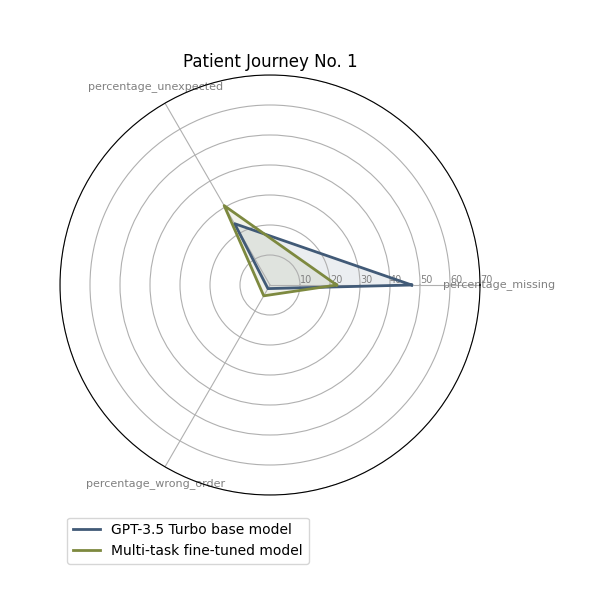
\includegraphics[width=0.3\textwidth]{bachelor_thesis/images/activites_pj1.png}}
  \subfigure[Patient Journey Nr. 2]{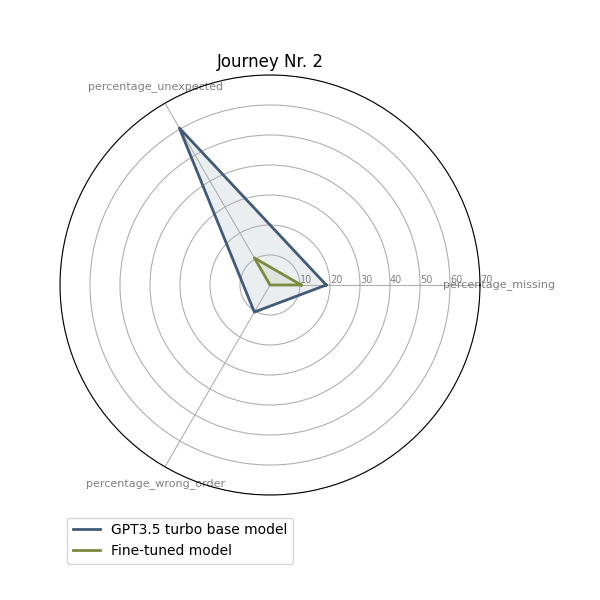
\includegraphics[width=0.3\textwidth]{bachelor_thesis/images/activites_pj2.png}}
  \subfigure[Patient Journey Nr. 3]{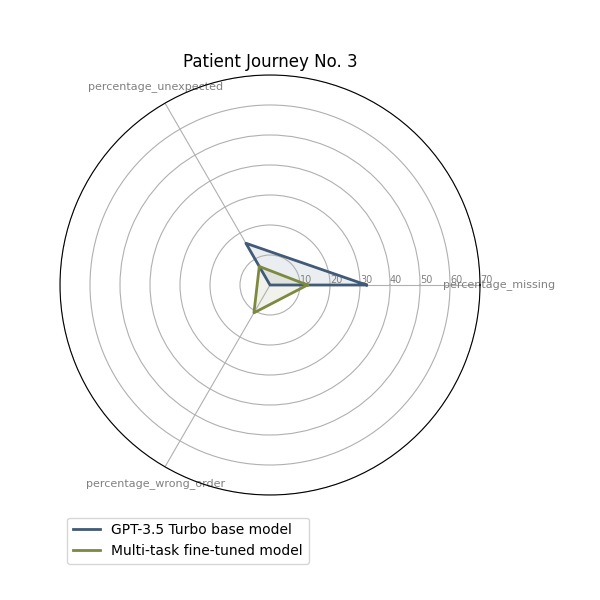
\includegraphics[width=0.3\textwidth]{bachelor_thesis/images/activites_pj3.png}}
  \subfigure[Patient Journey Nr. 4]{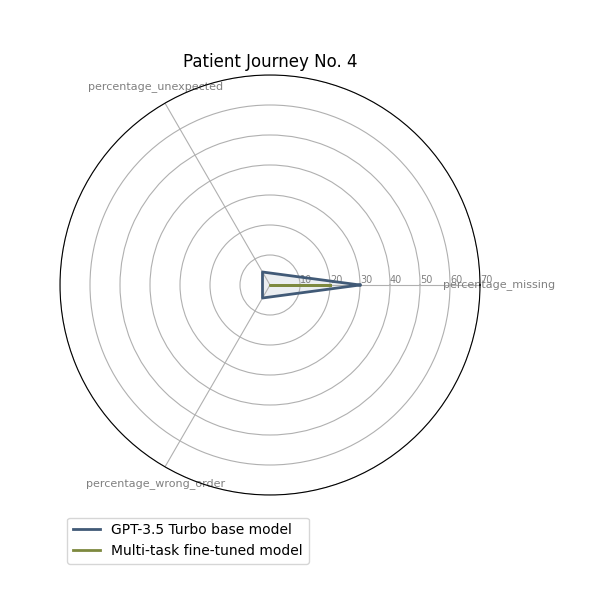
\includegraphics[width=0.3\textwidth]{bachelor_thesis/images/activites_pj4.png}}
  \subfigure[Patient Journey Nr. 5]{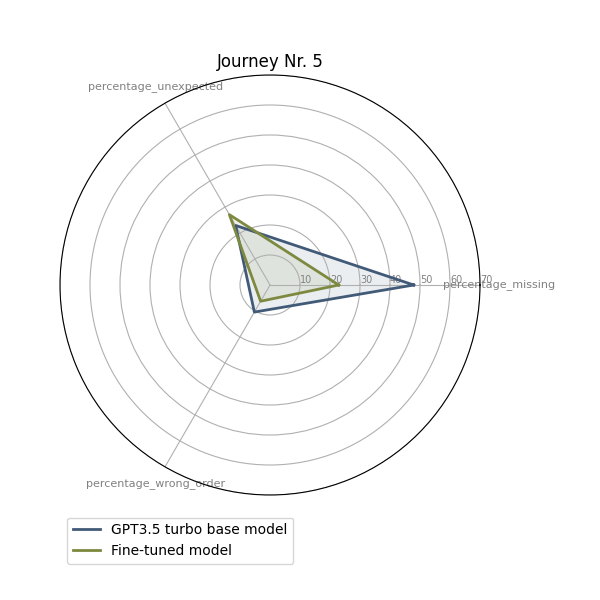
\includegraphics[width=0.3\textwidth]{bachelor_thesis/images/activites_pj5.png}}
  \caption{Radar Plots comparing the extraction results of GPT-3.5 Turbo and the Multi-Task Fine-Tuned model for Patient Journey 1-5~\ref{apx:pjs} for the task \quotes{Activity Labelling}}
  \label{fig:eval_activities_rad}
\end{figure}
Figure~\ref{fig:eval_activities_bar} illustrates the performance of both models across all patient journeys in a bar plot. Each bar represents the error rate in one of the metrics and the bars of the same metric for, each Patient Journey of base- and fine-tuned model respectively, overlap each other. A smaller amplitude is desirable. Although the fine-tuned model performed slightly worse in some metrics, its overall supremacy is evident. Especially with Patient Journey~1,2 and 4 the difference is clearly notable.  We make the following observations:
\begin{enumerate}
    \item \emph{Wrong Order} is the error type with the least occurrences across both models. On an average, there are more \emph{Missing Activity} errors than \emph{Unexpected Activity} errors. This indicates, that both model tend to rather not include relevant event than include irrelevant or imaginary events.
    \item The quality of the results is as diverse as the Patient Journeys.
    \item Patient Journey Nr.~5, which we assess to be the most challenging, has the highest overall error rate. This hints to a correlation between lacklustre structure in the Patient Journeys and worse quality of the event log.
    \item The multi-task fine-tuned model overall outperforms the base-model, though not consistently
\end{enumerate}

\begin{figure}
    \centering
    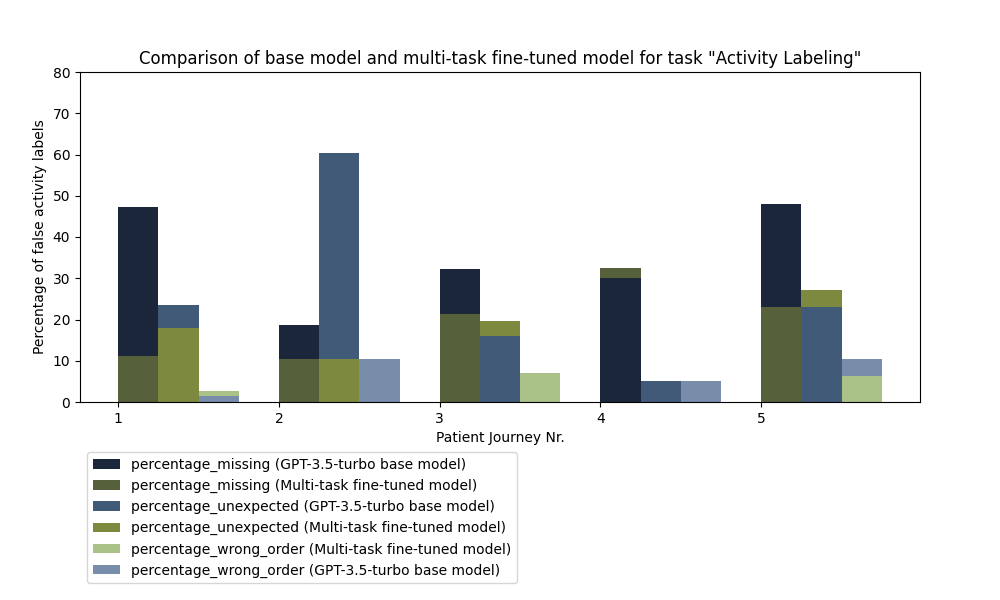
\includegraphics[width=\textwidth]{bachelor_thesis/images/activities_all.png}
    \caption{Bar Plot comparing the extraction results of GPT-3.5 Turbo and the Multi-Task Fine-Tuned model across all Patient Journeys~\ref{apx:pjs} for the task \quotes{Activity Labelling}} 
    \label{fig:eval_activities_bar}
\end{figure}

\paragraph{Event Type Classification} \autoref{fig:eval_event_types} shows the performance of both models across all patient journeys in a bar plot. Each bar represents the percentage of incorrectly classified event types.It is clear, that GPT-3.5 performs better on nearly every Patient Journey. This can have various reasons, like an under-representation of certain event types in the training data. We discuss the mater in \autoref{sec:discussion}. The gap between the two models is rather small, to a point where it can be almost considered negligible. Fine-tuning the model definitely did not increase the quality of the extraction results in this task. However, they are almost as good as the base models while not receiving examples in few-shot prompts with every request to the API. We discuss the matter of token consumption in \autoref{sec:eval_other}.
\begin{figure}
    \centering
    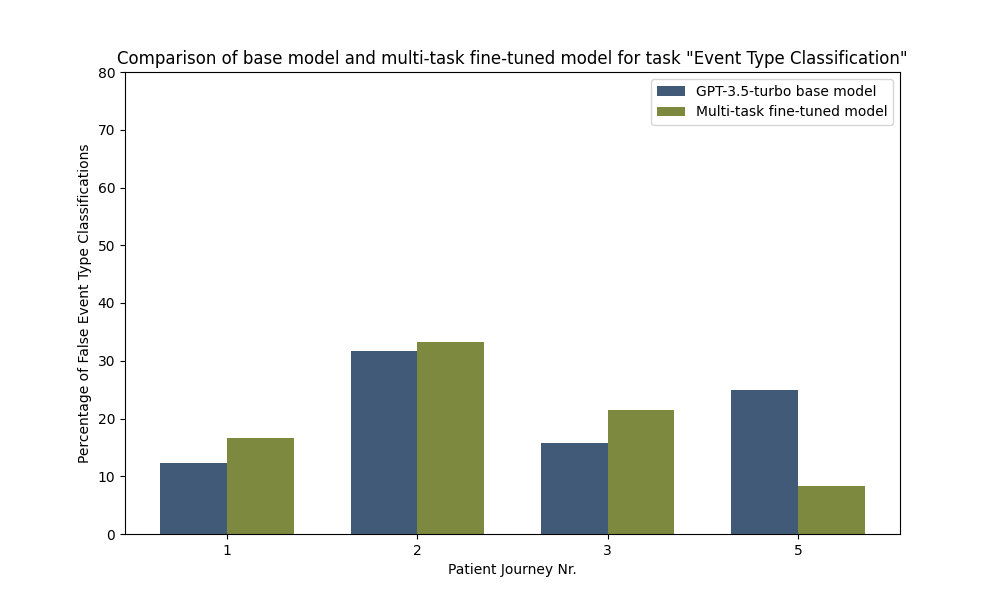
\includegraphics[width=\textwidth]{bachelor_thesis/images/event_types_all.png}
    \caption{Bar Plot comparing the extraction results of GPT-3.5 Turbo and the Multi-Task Fine-Tuned model across all Patient Journeys~\ref{apx:pjs} for the task \quotes{Event Type Classification}}
    \label{fig:eval_event_types}
\end{figure}

\paragraph{Timestamp Extraction}
The final task we trained the multi-task fine-tuned model for is extracting timestamps. \autoref{fig:eval_time} presents the ratio of incorrectly classified time stamps for both GPT-3.5 Turbo and the fine-tuned model. A smaller amplitude is desirable. We make the following observations:
\begin{enumerate}
    \item The error rate is considerably in this metric is higher than any other. This reflects our initial assessment, that the extraction of timestamps is the most difficult task out of the ones we evaluate in this thesis.
    \item the multi-task fine-tuned model achieved a better quality in almost every scenario. Especially the simpler Patient Journeys 2 and 4 were processed noticeably better. This indicates, that even the fine-tuned model struggles with the less well-structured description of time specifications and events with strong temporal relations.
\end{enumerate}
\begin{figure}
    \centering
    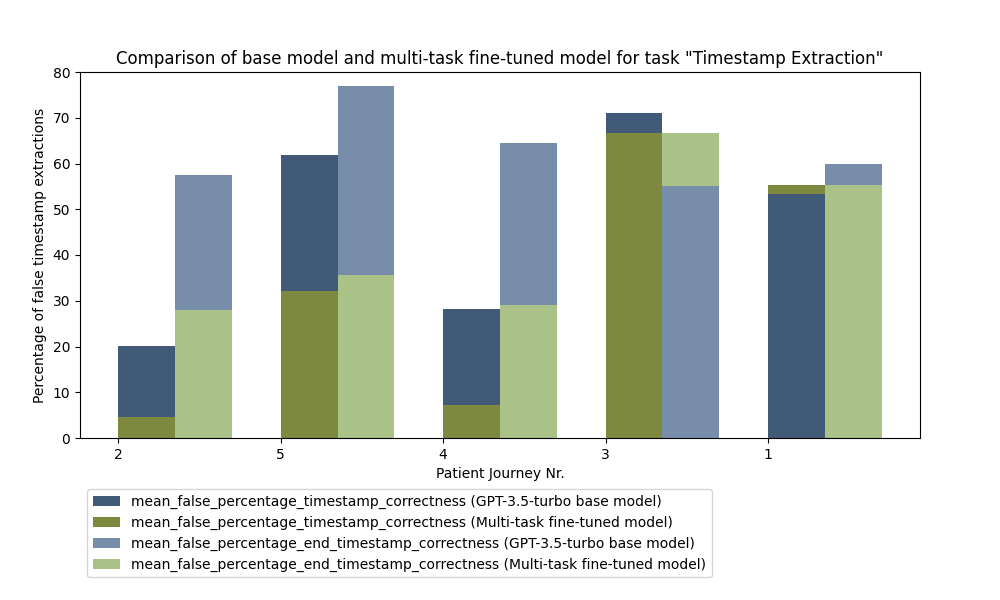
\includegraphics[width=\textwidth]{bachelor_thesis/images/timestamp_all.png}
    \caption{Bar Plot comparing the extraction results of GPT-3.5 Turbo and the Multi-Task Fine-Tuned model across all Patient Journeys~\autoref{apx:pjs} for the task \quotes{Timestamp Extraction}}
    \label{fig:eval_time}
\end{figure}


\subsubsection{Single-Task Fine-Tuned Model}\label{sec:eval_single}
The plots in \autoref{fig:eval_activities_single_rad} show comparisons of base model and single-task fine-tuned model in all three metrics for each Patient Journey individually. The axes each display the error rate in the extraction results the models achieved. A smaller amplitude is desirable.\\
\begin{figure}
  \centering
  \subfigure[Patient Journey Nr. 1]{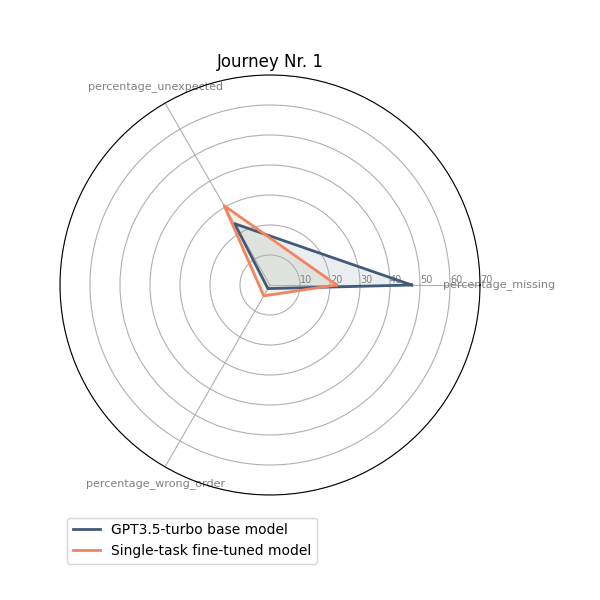
\includegraphics[width=0.3\textwidth]{bachelor_thesis/images/activites_pj1-single.png}}
  \subfigure[Patient Journey Nr. 2]{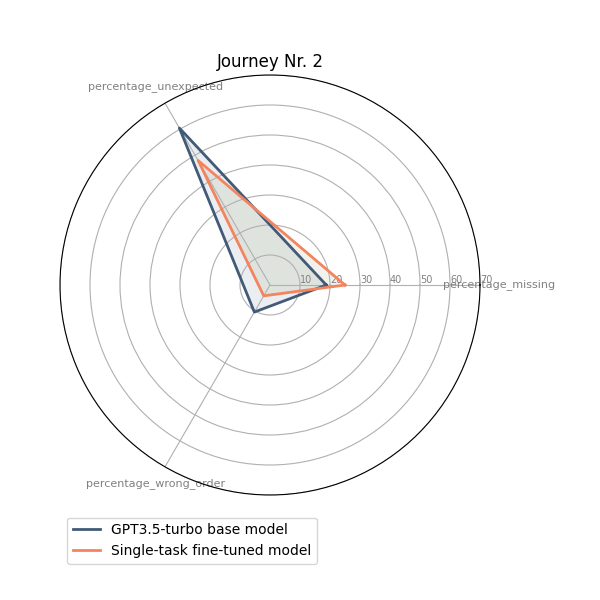
\includegraphics[width=0.3\textwidth]{bachelor_thesis/images/activites_pj2-single.png}}
  \subfigure[Patient Journey Nr. 3]{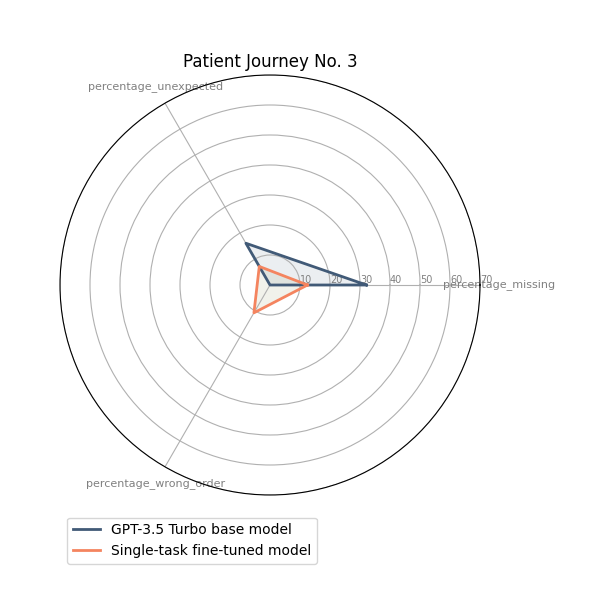
\includegraphics[width=0.3\textwidth]{bachelor_thesis/images/activites_pj3-single.png}}
  \subfigure[Patient Journey Nr. 4]{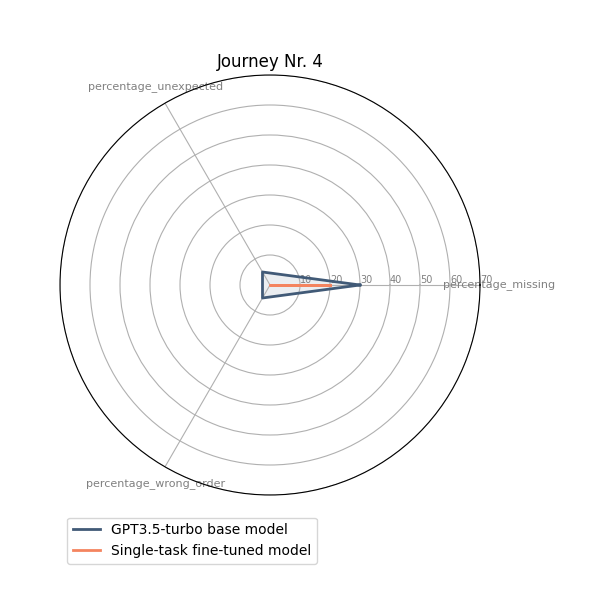
\includegraphics[width=0.3\textwidth]{bachelor_thesis/images/activites_pj4-single.png}}
  \subfigure[Patient Journey Nr. 5]{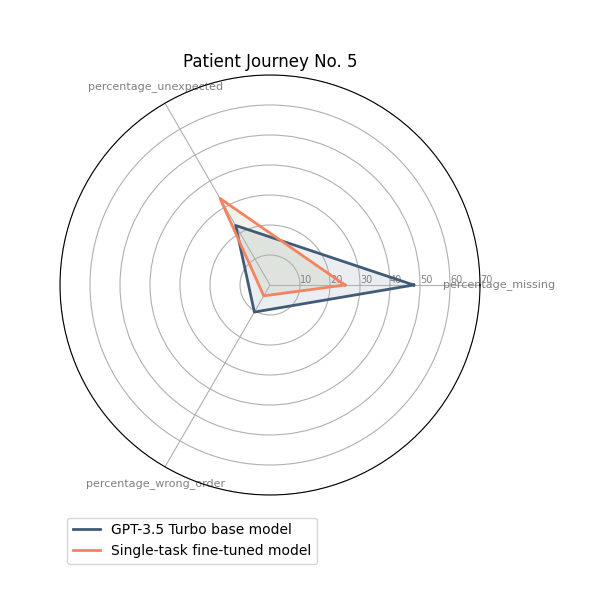
\includegraphics[width=0.3\textwidth]{bachelor_thesis/images/activites_pj5-single.png}}
  \caption{Radar Plots comparing the extraction results of GPT-3.5 Turbo and the Single-Task Fine-Tuned model for Patient Journey 1-5~\ref{apx:pjs} for the task \quotes{Activity Labelling}}
  \label{fig:eval_activities_single_rad}
\end{figure}
\autoref{fig:eval_activities_all_bar} illustrates the performance of both models across all patient journeys in a bar plot. Each bar represents the error rate in one of the metrics and the bars of the same metric for, each Patient Journey of base- and fine-tuned model respectively, overlap each other. A smaller amplitude is desirable. The fine-tuned model consistently scores better in the \emph{missing activity} metric, but only occasionally outperforms the base model in any other metric.
\begin{figure}
    \centering
    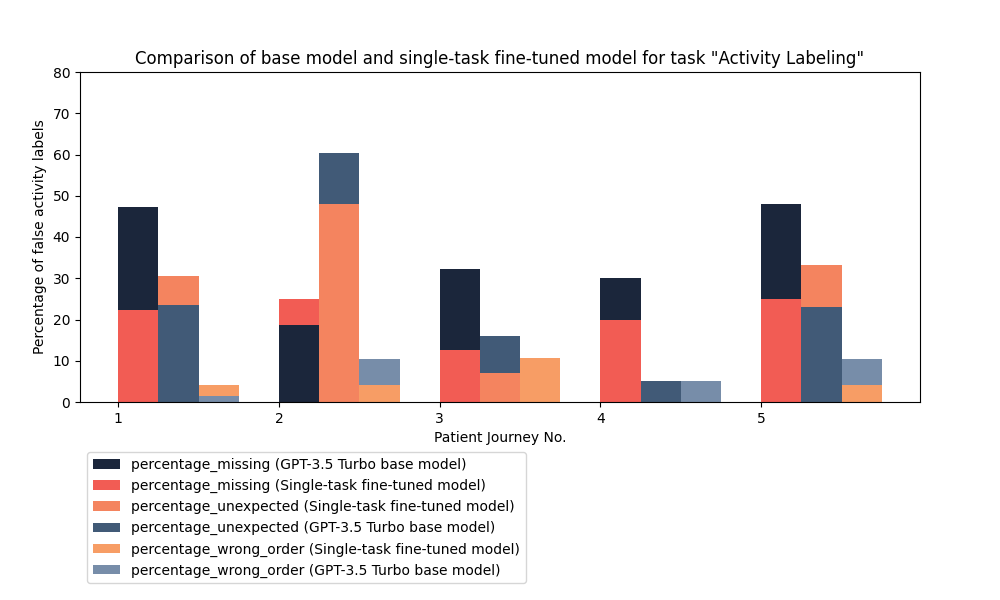
\includegraphics[width=\textwidth]{bachelor_thesis/images/activites_all-single.png}
    \caption{Bar Plot comparing the extraction results of GPT-3.5 Turbo and the Single-Task Fine-Tuned model across all Patient Journeys~\ref{apx:pjs} for the task \quotes{Activity Labelling}} 
    \label{fig:eval_activities_all_bar}
\end{figure}

\subsubsection{Comparison of Fine-Tuned Models}
Lastly, we compare the results of the two fine-tuned models in their mutual task \quotes{Activity Labelling}. As you can see in \autoref{fig:eval_activities_all_comparison_bar} the multi-task fine-tuned model performs better in 8 out of 15 measurements and the single-task fine-tuned model performs better in the other 7 measurements. All models performed notably good on Patient Journey 3 and 4, so these seem to be the easiest for an LLM to extract information from. The single-task fine-tuned model got the best scores for both of them. This indicates, that the specialisation on one task increases the performance in easier conditions while not increasing the performance under more difficult conditions. We further discuss this in~\autoref{sec:discussion}.

\begin{figure}
    \centering
    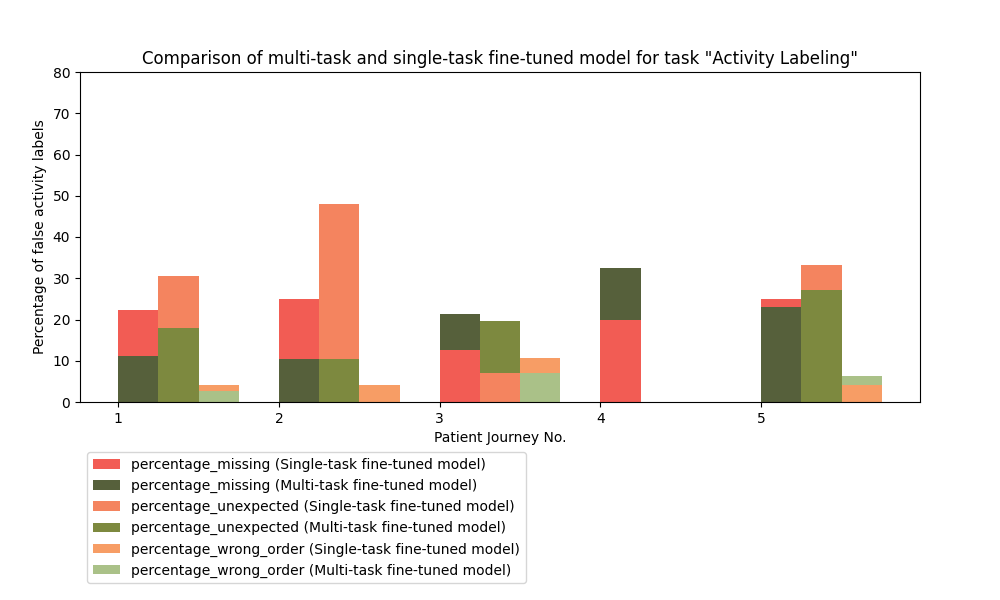
\includegraphics[width=\textwidth]{bachelor_thesis/images/activites_all-single_vs_multi.png}
    \caption{Bar Plot comparing the extraction results of multi-task and single-task fine-tuned model across all Patient Journeys~\ref{apx:pjs} for the task \quotes{Activity Labelling}} 
    \label{fig:eval_activities_all_comparison_bar}
\end{figure}
